
\section{Transition Radiation Detector} \label{TRDSection}

% Definition of Transition radiation and the Characters of Transition Radiation 
The TRD can separate different particles based on the transition radiation emitted. Transition radiation is emitted when a relativistic charged particle goes through the boundary between two different mediums with different dielectric constants \cite{TransitionRadiation_Ginzburg1945}. The emitted radiation is produced due to the different solutions of Maxwell's equations of the electric and magnetic fields of the moving charged particle in these two mediums, so photons have to be emitted when the particle crosses the boundary. The intensity of the emitted photon is proportional to the Lorentz factor $\gamma$, so for a relativistic charged particle, the emitted transition radiation photons have wavelengths in the X-ray range of the electromagnetic spectrum and their direction is mostly forward. The angle between transition radiation and particle path is proportional to $1/\gamma$.    \par


% AMS TRD
The AMS-02 experiment has a transition radiation detector placed on the top of the experiment between the tracker layer one and the upper TOF layer \cite{AMS02TRDPaper1, AMS02TRDPaper2}. The TRD has 5248 proportional straw tubes; each one has a 6 mm diameter and a maximum length of 2 m. The straw tubes have double-layer kapton-aluminum foil walls of 72 $\mu$m in thickness and at their center there is a 30 $\mu$m gold-plated tungsten wire. The tubes are filled with a xenon (Xe) and carbon dioxide (CO2) gas mixture, which is supplied by two storage tanks (5 kg $\rm CO_2$ and 49 kg $\rm Xe$). When a charged particle goes through the straw tube it ionizes the $\rm{Xe}$ atoms and the produced electrons drift towards the anode wire creating an avalance of ionization proportional to the energy loss of the particle. Finally, a signal is induced on the anode wire. The $\rm CO_2$ quenches the environment and reset it to its initial state. So far, no detectable large leak in the AMS-02 TRD gas system has been observed. Due to gas diffusion across the tube walls, the loss of $\rm CO_2$ is around 0.47 g/day and the loss for $\rm Xe$ is negligible. This ensures that the TRD can be stably operated until 2039.  \par

The TRD tubes are assembled in 328 modules and one module has 16 tubes. Furthermore, all these modules are mounted in 20 layers. Twelve layers are placed along the Y axis in the middle of TRD, four layers are placed along the x-axis on top, and four layers along the x-axis are on the bottom. In figure \ref{TRDConstruction}, the TRD and its support structure are shown.  \par

\begin{figure}[t]
\centering
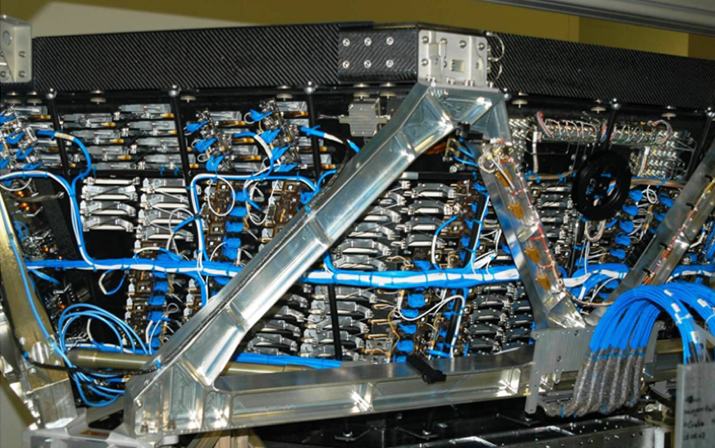
\includegraphics[width=0.8\textwidth, height=0.4\textheight ]{Figures/chapter3/TRD/TRDConstruction.png}
\caption[The TRD and its support structure during construction.]{The TRD and its support structure during construction \cite{AMSWebside}.}
\label{TRDConstruction}
\end{figure}

% TRD transition radiation 
Figure \ref{TRDdEdXPlot} shows an illustration where an electron and a proton go through one TRD layer. The upper part of the layer is a 20 mm thick fleece radiator, which consists of 10 $\rm{\mu m}$ thick polypropylene or polyethylene fibers. The lower part of the layer is made of straw tubes. When a relativistic charged particle goes through the radiator, transition radiation may be produced. For example, the ${\rm{d}}E/{\rm{d}}X$ signal can be recorded after a proton traverses the layer. While an electron passes the layer, the transition radiation can also be collected in straw tubes. Figure \ref{TRDTubeEnergy} shows the energy distributions measured by TRD straw tubes for 60 GeV protons, pions, muons and 20 GeV electrons during a test beam at CERN. Due to the transition radiation emitted by electrons, there is an additional contribution from the transition radiation photons at around $\sim$10 keV in the electron's spectrum. \par

\begin{figure}[H] 
\centering   
\subfigure[] {
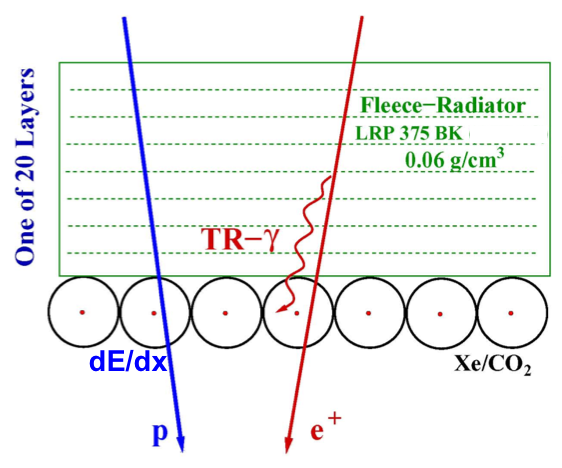
\includegraphics[width=0.47\columnwidth, height=0.28\textheight]{Figures/chapter3/TRD/TRDdEdX1.png} 
\label{TRDdEdXPlot}
}    
\subfigure[] { 
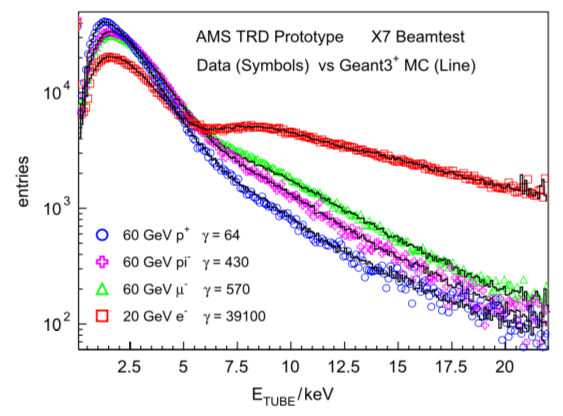
\includegraphics[width=0.47\columnwidth, height=0.25\textheight]{Figures/chapter3/TRD/TRDdEdX2.png}    
\label{TRDTubeEnergy}
}     
\caption[Illustration of the TRD separation between electrons and protons.]{Illustration of the TRD separation between electrons and protons: a) the transition radiation emitted by a positron while the proton can only produces the ${\rm{d}}E/{\rm{d}}X$ signals in the TRD \cite{AMSWebside}; b) the energy distributions measured by TRD straw tubes for 60 GeV protons, pions, muons and 20 GeV electrons during a beam test at CERN \cite{TRD_DEDXPaper}. }
\label{TRDdEdX} 
\end{figure}








